
%(BEGIN_QUESTION)
% Copyright 2012, Tony R. Kuphaldt, released under the Creative Commons Attribution License (v 1.0)
% This means you may do almost anything with this work of mine, so long as you give me proper credit

Two control loops are seen at work in this mixing tank.  The flow control loop regulates liquid flow into the tank, while the level control loop regulates liquid level inside the tank:

$$\includegraphics[width=15.5cm]{i03391x01.eps}$$

The following list shows the actions of the sensing and final control instruments for both loops:

\begin{itemize}
\item{} Flow transmitter = {\it direct} action (i.e. more flow = greater signal)
\item{} Flow valve = {\it air to open} 
\item{} Level transmitter = {\it direct} action (i.e. higher level = greater signal)
\item{} Level valve = {\it air to open}
\end{itemize}

Determine the proper controller actions ({\it direct} or {\it reverse}) for the FC and for the LIC.

\underbar{file i03391}
%(END_QUESTION)





%(BEGIN_ANSWER)

FC = {\bf reverse} action

LIC = {\bf direct} action

%(END_ANSWER)





%(BEGIN_NOTES)

{\bf This question is intended for exams only and not worksheets!}.

%(END_NOTES)


